\documentclass{beamer}

% For more themes, color themes and font themes, see:
% http://deic.uab.es/~iblanes/beamer_gallery/index_by_theme.html
%
\mode<presentation>
{
  \usetheme{Madrid}       % or try default, Darmstadt, Warsaw, ...
  \usecolortheme{default} % or try albatross, beaver, crane, ...
  \usefonttheme{serif}    % or try default, structurebold, ...
  \setbeamertemplate{navigation symbols}{}
  \setbeamertemplate{caption}[numbered]
} 

%\usepackage[english]{babel}
%\usepackage[utf8x]{inputenc}
\usepackage[russian]{babel}
\usepackage[utf8x]{inputenc}
\usepackage{chemfig}
\usepackage[version=3]{mhchem}
\usepackage{amssymb}
\usepackage[ampersand]{easylist}
\usepackage{graphicx}
\graphicspath{{pictures/}}
\DeclareGraphicsExtensions{.pdf,.png,.jpg}

% On Overleaf, these lines give you sharper preview images.
% You might want to `comment them out before you export, though.
\usepackage{pgfpages}
\pgfpagesuselayout{resize to}[%
  physical paper width=8in, physical paper height=6in]

% Here's where the presentation starts, with the info for the title slide
\title[Неконтролируемое обучение]{Кластеризация изображений по визуальному подобию с помощью вариационных автоэнкодеров}
\author{А. Коваленко}
\institute{ЮФУ}
\date{\today}

\newcommand\myitemize{\ListProperties(Hide=100, Hang=true, Progressive=3ex, Style*=$\star$ )}
\newcommand\myenumerate{\ListProperties(Space=2\baselineskip)}

\begin{document}

\begin{frame}
  \titlepage
\end{frame}

% These three lines create an automatically generated table of contents.
\begin{frame}{Содержание}
  \tableofcontents
\end{frame}

\section{Введение}

\subsection{Постановка задачи}
\begin{frame}{Введение}{Постановка задачи}
Разметка данных всегда трудоемкий процесс. Поэтому алгоритмы машинного обучения не требующие данного этапа актуальны. Класс вариационных автоэнкодеров позволяет решить данную проблему.\\

\begin{block}{Поставим задачу:}
	Пусть имеется набор изображений: $$X = \{I_m\}_{m = 1}^{N}$$
	Требуется разбить данный набор на \textit{K} классов и ввести операцию сравнения.\\
	Для произвольного изображения найдем \textit{M} схожих объектов из множества \textit{X}, отсортированных по убыванию визуального подобия:
	$$I_{input} \notin X,  S = \{I_{m_k}\}_{k=1}^M$$
\end{block}

\end{frame}

\subsection{Обзор подходящих алгоритмов}



\begin{frame}{Введение}{Обзор подходящих алгоритмов}

Для решения поставленной задачи могут подойти следующие подходы неконтролируемого обучения и обучения с подкреплением:
\begin{itemize}
	\item Сиамские нейронные сети
	\item Ключевые точки (не является алгоритмом машинного обучения)
	\item Автоэнкодеры
\end{itemize}

\end{frame}

\begin{frame}{Введение}{Обзор подходящих алгоритмов}

Для решения поставленной задачи могут подойти следующие подходы неконтролируемого обучения и обучения с подкреплением:
\begin{itemize}
	\item Сиамские нейронные сети
	\item Ключевые точки (не является алгоритмом машинного обучения)
	\begin{block}
		\item Автоэнкодеры
	\end{block}
\end{itemize}

\end{frame}

\section{Автоэнкодеры}

\subsection{Принцип работы}


\begin{frame}{Автоэнкодеры}{Принцип работы}

\begin{block}{Определение:}
	\textbf{Автоэнкодеры} --- это нейронные сети прямого распространения, которые восстанавливают входной сигнал на выходе.
\end{block}

\begin{figure}[h]
	\center{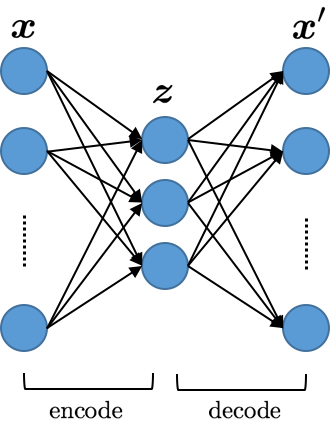
\includegraphics[scale=0.7]{ae}}
	\caption{Общая схема автоэнкодера}
	\label{fig:ae}
\end{figure}

\end{frame}

\begin{frame}{Автоэнкодеры}{Принцип работы}

\begin{minipage}{0.4\textwidth}
\begin{flushleft}
	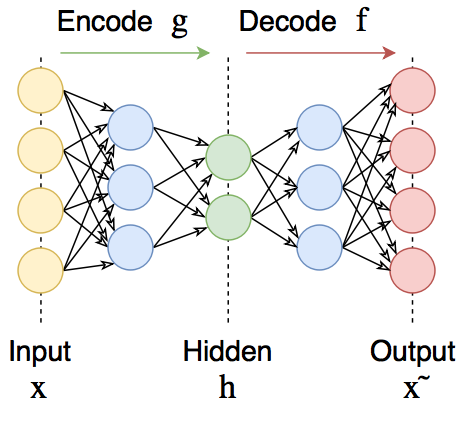
\includegraphics[scale=0.35]{ae_1}
\end{flushleft}
\end{minipage}
\hfill
\begin{minipage}{0.4\textwidth}
\begin{center}
		$$g - \text{энкордер}, f - \text{декодер},$$
		$$x - \text{сигнал}, h - \text{код сигнала}$$
		$$h = g(x), x = f(h)$$
		\begin{equation}\label{eq:aim_func}
			x = f(g(x))
		\end{equation}
\end{center}
\end{minipage}

\end{frame}

\subsection{Разряженные автоэнкодеры}

\begin{frame}{Автоэнкодеры}{Разряженные автоэнкодеры}
Автоэнкодер при обучении стремится аппроксимировать \text{функцию ~(\ref{eq:aim_func}):} $$x = f(g(x)),$$ минимизируя заданный функционал ошибки:
\begin{equation}
\min_{\omega} L(x, f(g(x))),
\end{equation}
где $\omega$ - параметры автоэнкодера

\begin{block}{Определение:}
	\textbf{Разряженным} называется автоэнкодер, для которого критерий обучения включает также минимизацию разреженности $\Omega(h)$ на кодовом слове $h$:
	$$\min_{\omega} L(x, f(g(x))) + \Omega(h),$$
	где $\Omega(h)$ - обычный регуляризатор (пусть $L_1$), $\Omega(h) = \lambda*\|h\|$
\end{block}

\end{frame}

\subsection{Вариационные автоэнкодеры}

\begin{frame}{Автоэнкодеры}{Вариационные автоэнкодеры}
Рассмотрим работу декодера как некоторый процесс генерации данных $X$, зависящий от скрытых переменных $Z$ - случайных величин.\\
Пусть:
\begin{itemize}
	\item $p(X)$ - вероятностное распределение изображений
	\item $p(Z)$ - вероятностное распределение скрытых переменных
	\item $$
\end{itemize}
\end{frame}

\end{document}
